\documentclass{mwart}
\usepackage{multicol}
\usepackage{polski} % Pozwala na użycie polskiego. Ustawia między innymi fontenc na T1
\usepackage[utf8]{inputenc} % Informuje o kodowaniu
\usepackage{enumitem}
\usepackage{xcolor}
\usepackage{xcolor}% http://ctan.org/pkg/xcolor
\usepackage{hyperref}
\usepackage{listings}
\usepackage{float} % Ustawianie obrazów
\usepackage[caption = false]{subfig} % Wiele obrazów w jednej figurze
\definecolor{LinkColor}{HTML}{1d5cc1}
\renewcommand{\labelitemi}{\textbullet} % Zmiana symbolu wliczeń

\lstset{
  basicstyle=\ttfamily,
  columns=fullflexible,
  breaklines=true,
  postbreak=\mbox{\textcolor{red}{$\hookrightarrow$}\space},
}

\definecolor{LinkColor}{HTML}{1d5cc1}

\usepackage{tabto}

\usepackage{graphicx} % Pakiet do obrazów
\graphicspath{ {./Obrazy/} } % Folder, z którego będą brane obrazy

% Nie twórz nowych stron
\usepackage{etoolbox}
\makeatletter
% \patchcmd{\chapter}{\if@openright\cleardoublepage\else\clearpage\fi}{}{}{}
\makeatother

\newcommand{\paragraphnl}[1]{\paragraph{#1} \mbox{} \\} % Paragraf z nową linią

\title{Projekt indywidualny ----  Raport końcowy}
\author{Krzysztof Dąbrowski}
\date{\today}

\begin{document}
\maketitle{}

\tableofcontents{}

% \section{Ostateczny projekt klas}

\section{Opis projektu}
Celem projektu jest napisanie aplikacji webowej pozwalającej na planowanie semestru studentom korzystającym z systemu \textit{USOS}.
W tym celu został wykonany program w języku C\# w oparciu o framework \textit{ASP.net MVC}. Dzięki temu możliwe było łatwe wydzielenie warstw widoku, modelu i kontrolerów.

Aplikacja została opublikowana w Internecie z wykorzystaniem chmury \textit{Microsoft Azure} co jest dokładniej opisanie w punkcie \ref{sec:chmura}.

\subsection{Wzorzec MVC}
Aby wprowadzić spójność wśród klas aplikacji, wyznaczyć zakres funkcji realizowany przez dany element oraz sprecyzować zasady komunikacji architektura
projektu będzie bazować na wzorcu Model View Controller.
Wyraźny podział elementów zaproponowany przez ten wzorzec będzie bezpośrednio realizowany przez podział klas na odpowiadające przestrzenie nazw.

Klasy z przestrzeni Models reprezentują automaty zajęcia uczelniane, plan zajęć oraz fragmenty przetwarzanego dokumentu.

Klasy z przestrzeni Views są odpowiedzialne za wygląd i wyświetlanie interfejsu programu. Składają się na nie pliki \texttt{.schtml}, które są przetwarzane dynamicznie do plików \texttt{.html} zwracanych do przeglądarki.

Klasy z przestrzeni Controllers wykonują walidacje po stronie serwera. Kontrolują również przejście do kolejnych części aplikacji poprzez przekierowania oraz zwracanie widow.

\section{Opis problemu}
Celem aplikacji jest pomoc w rozwiązaniu realnego problemu jakim jest wybór odpowiednich grup na zajęcia akademickie przez studentów korzystających z systemu \textit{USOS}.

Na wielu uczelniach nie ma podziału na grupy dziekańskie, dla których jest odgórnie układany plan. Zamiast tego student jest odpowiedzialny za własnoręczne skonfigurowanie planu na przyszłe semestry. 

Wygląd przykładowego planu dla kierunku Geografia prowadzonego na Uniwersytecie Warszawskim jest przedstawiony na rysunku \ref{fig:przykladowyPlan}.

Łatwo zauważyć, że tak przedstawiony plan może być przytłaczający i nieczytelny. Z tego powodu mój projekt pozwala na wczytanie planu po podaniu linku oraz wyświetla plan gdzie widoczne są jednocześnie jedynie zajęcia z wybranych grup.

Dzięki temu student może przeprowadzić wizualizację różnych odpowiadających mu konfiguracji planu. Dodatkowo zajęcia różnych typów są zaznaczone innymi kolorami co daje dodatkowe informacje wizualne.

\begin{figure}[h]
    \centering
    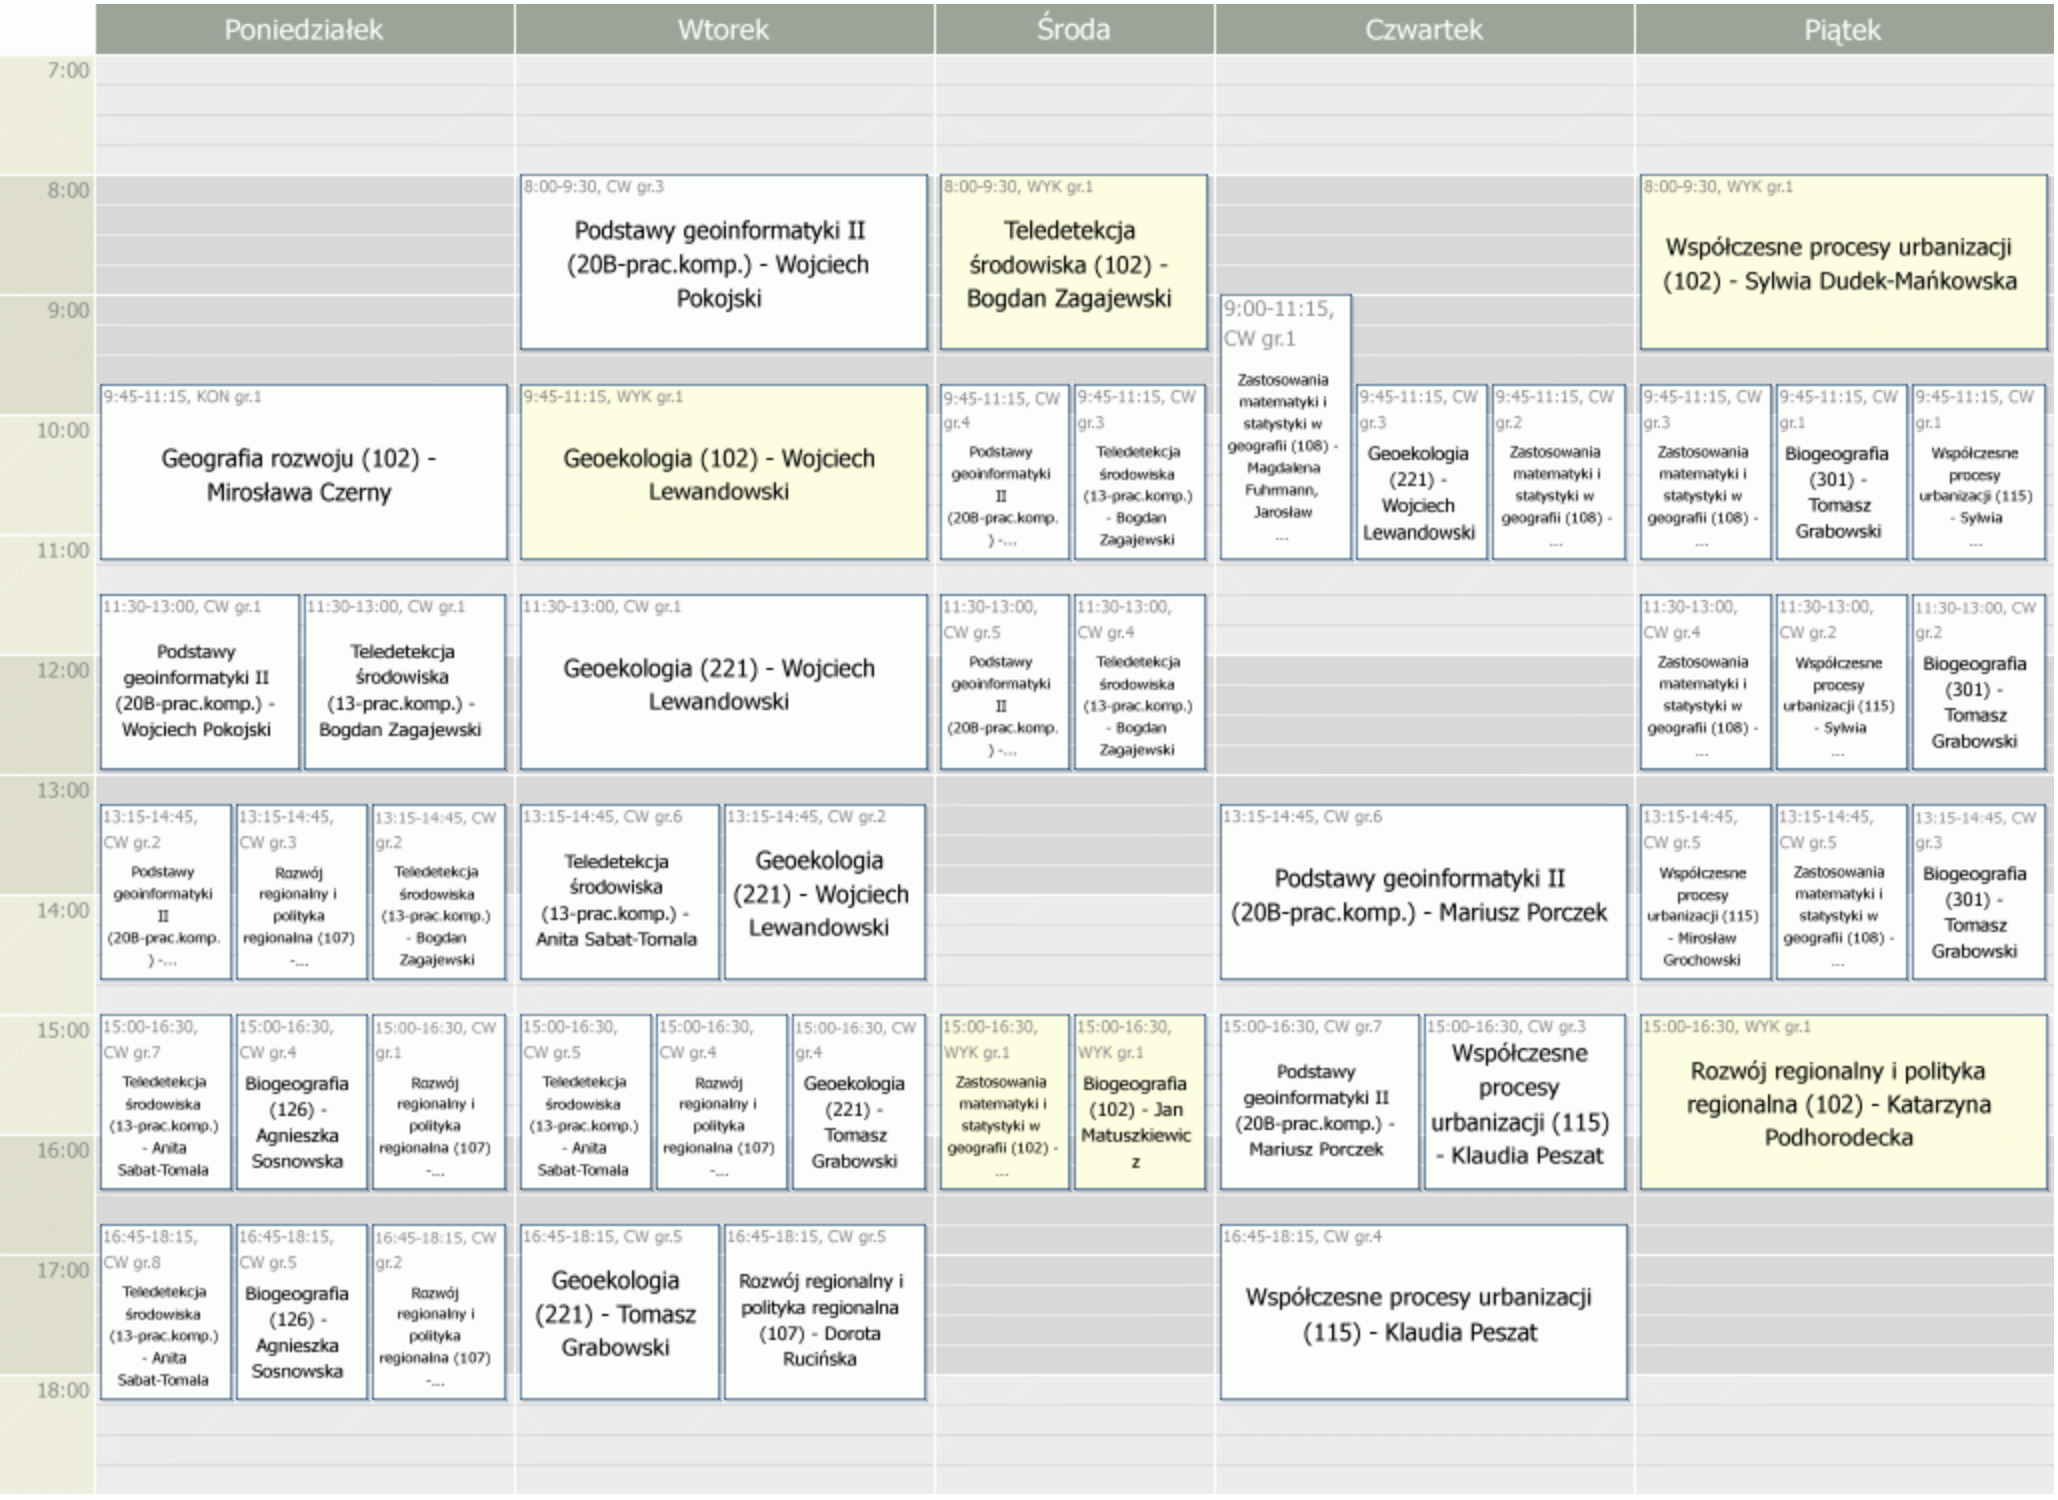
\includegraphics[width=13cm]{Example_plan}
    \caption{Modele}
    \label{fig:przykladowyPlan}
\end{figure}


\newpage{}
\section{Projekt klas}
Projekt klas reprezentujący model planu jest przedstawia diagram klas zawarty na figurze \ref{fig:klasy}.

\begin{figure}[H]
    \centering
    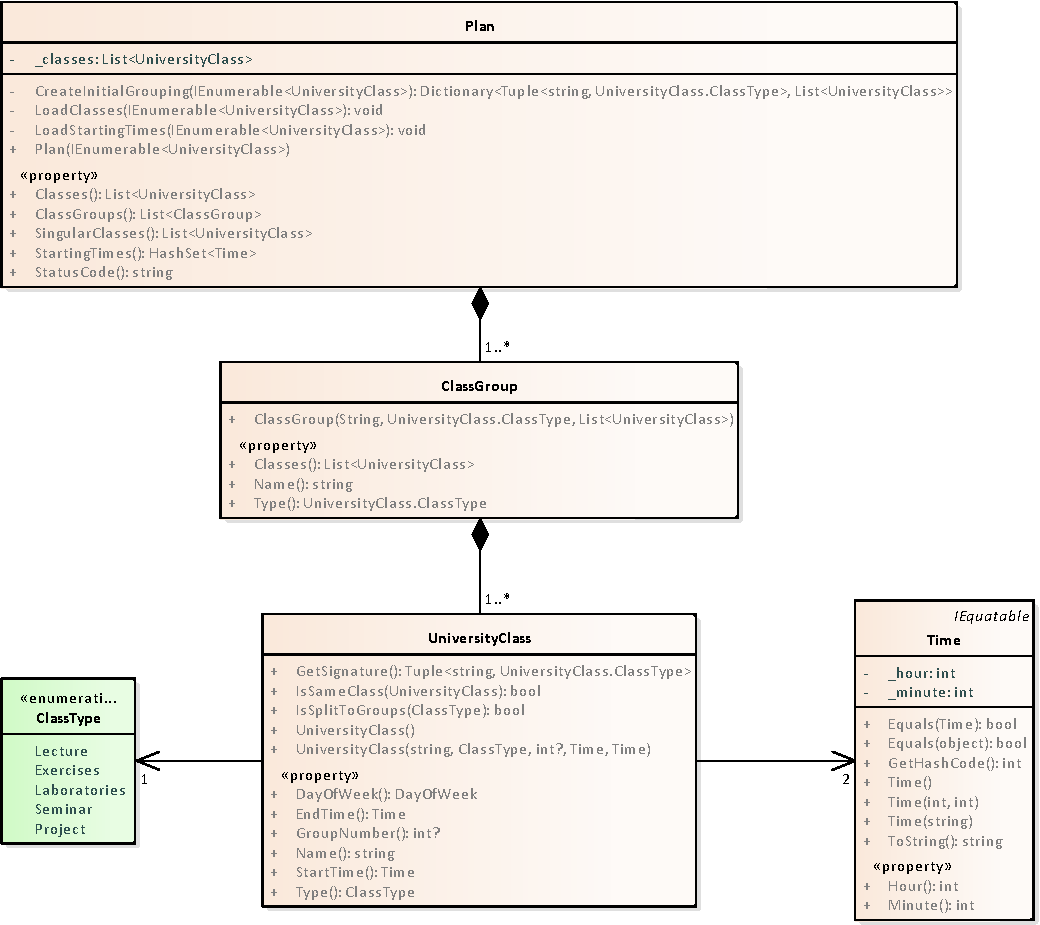
\includegraphics[width=13cm]{klasy.pdf}
    \caption{Modele}
    \label{fig:klasy}
\end{figure}

\section{Prezentacja działania}
Po przejściu na witrynę główną aplikacji użytkownik zobaczy ekran główny opisujący po krótce aplikację oraz pozwalający na przejście do ekranu wczytania planu. Ekran ten jest widoczny na figurze \ref{fig:ekranStartowy}.

\begin{figure}[h]
    \centering
    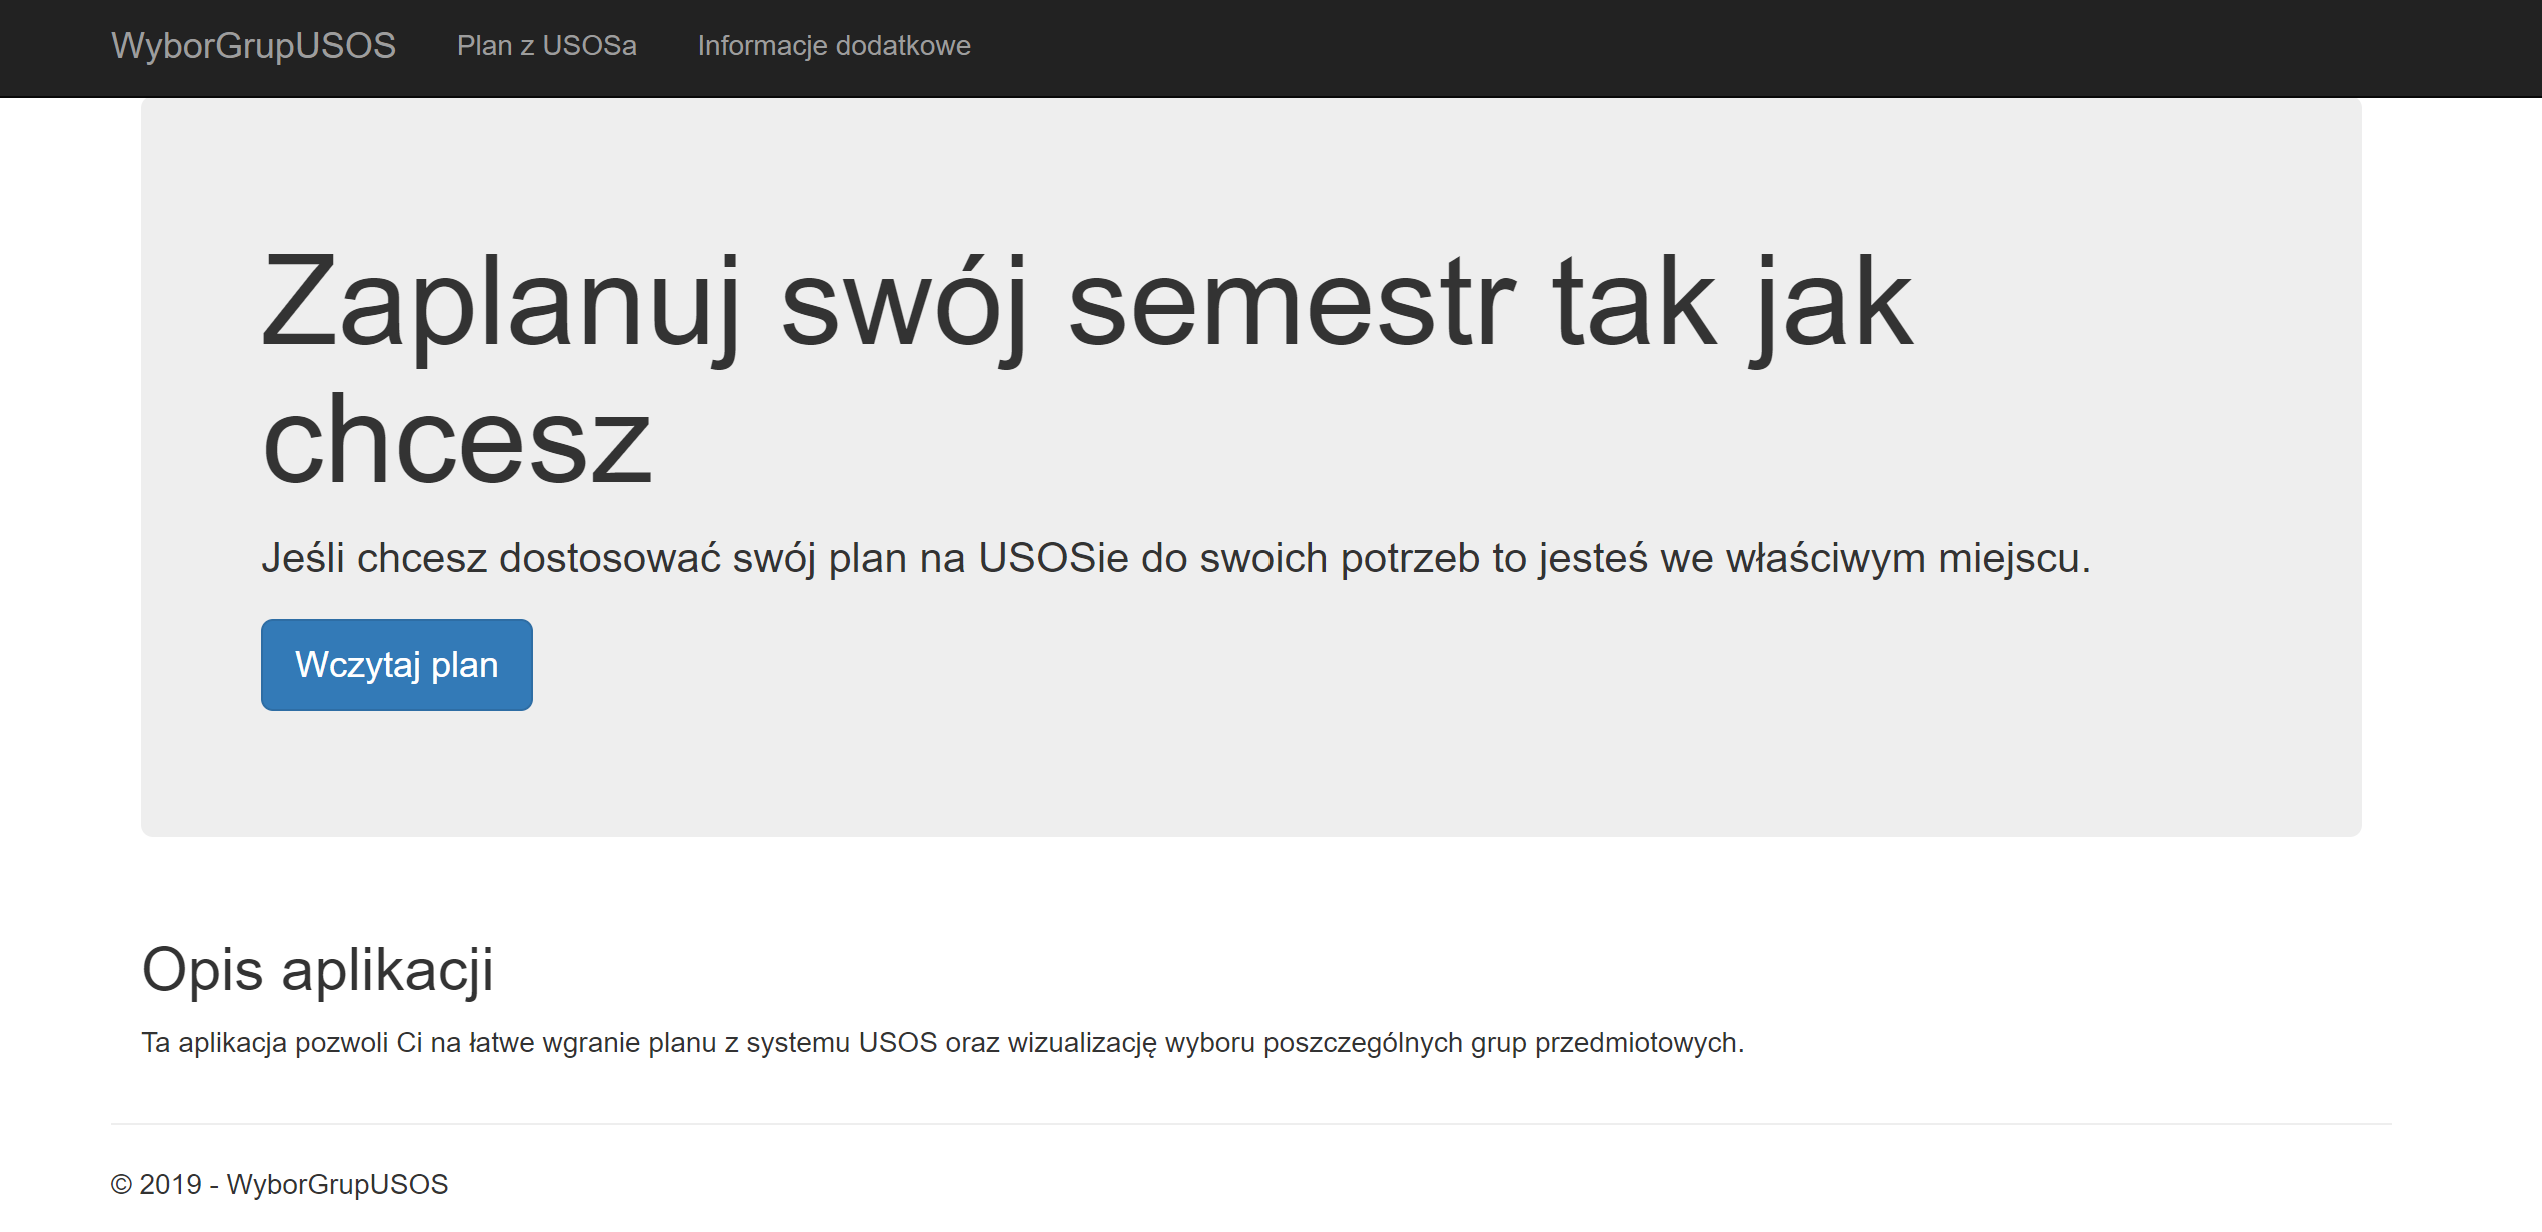
\includegraphics[width=13cm]{Ekran_startowy}
    \caption{Ekran startowy}
    \label{fig:ekranStartowy}
\end{figure}

Po przejściu dalej zostanie wyświetlony ekran pozwalający na przekazanie aplikacji linku do planu. Ekran zawiera też rozwijaną część opisjącą dokładniej szczegóły działania oraz wskazujący przykładowy plan. Możliwe jest wczytanie wskazanego planu lub plany przykładowego. Ekran ten przedstawiają figury \ref{fig:ekranWczytaniaZwiniety} i \ref{fig:ekranWczytaniaRozwiniety}.

\begin{figure}[h]
    \centering
    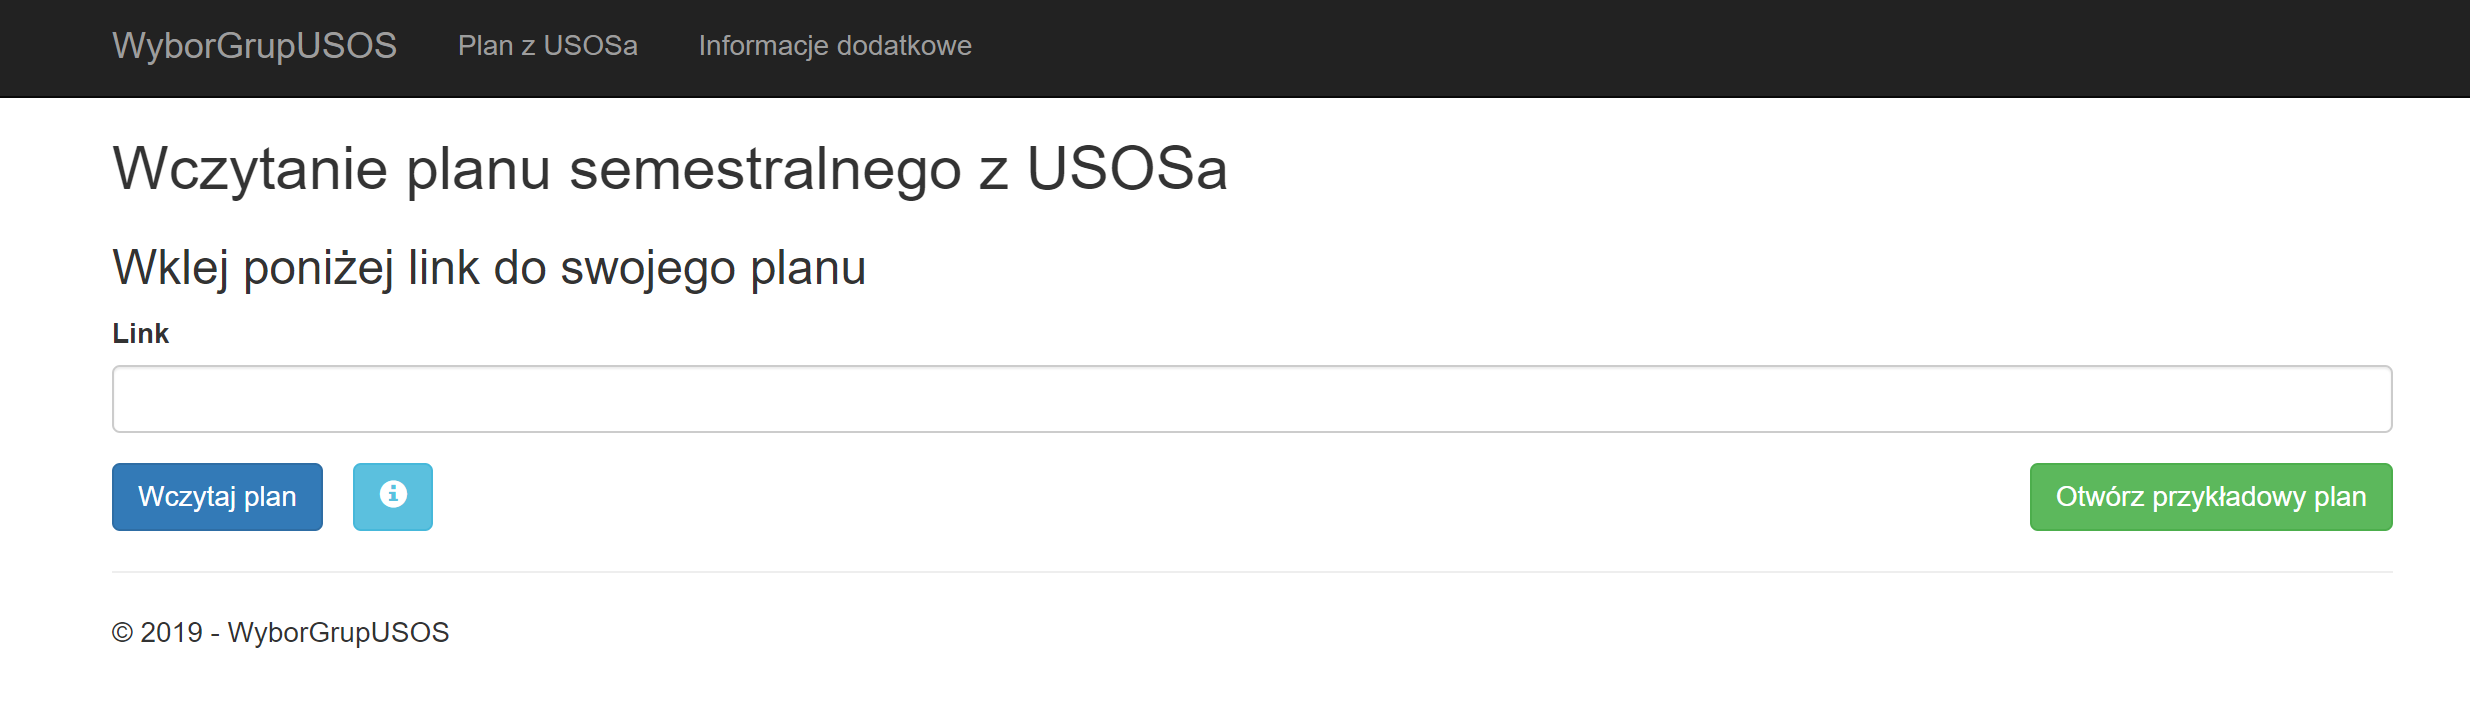
\includegraphics[width=13cm]{Ekran_wczytania_zwiniety}
    \caption{Ekran wczytania bez dodatkowych informacji}
    \label{fig:ekranWczytaniaZwiniety}
\end{figure}

\begin{figure}[h]
    \centering
    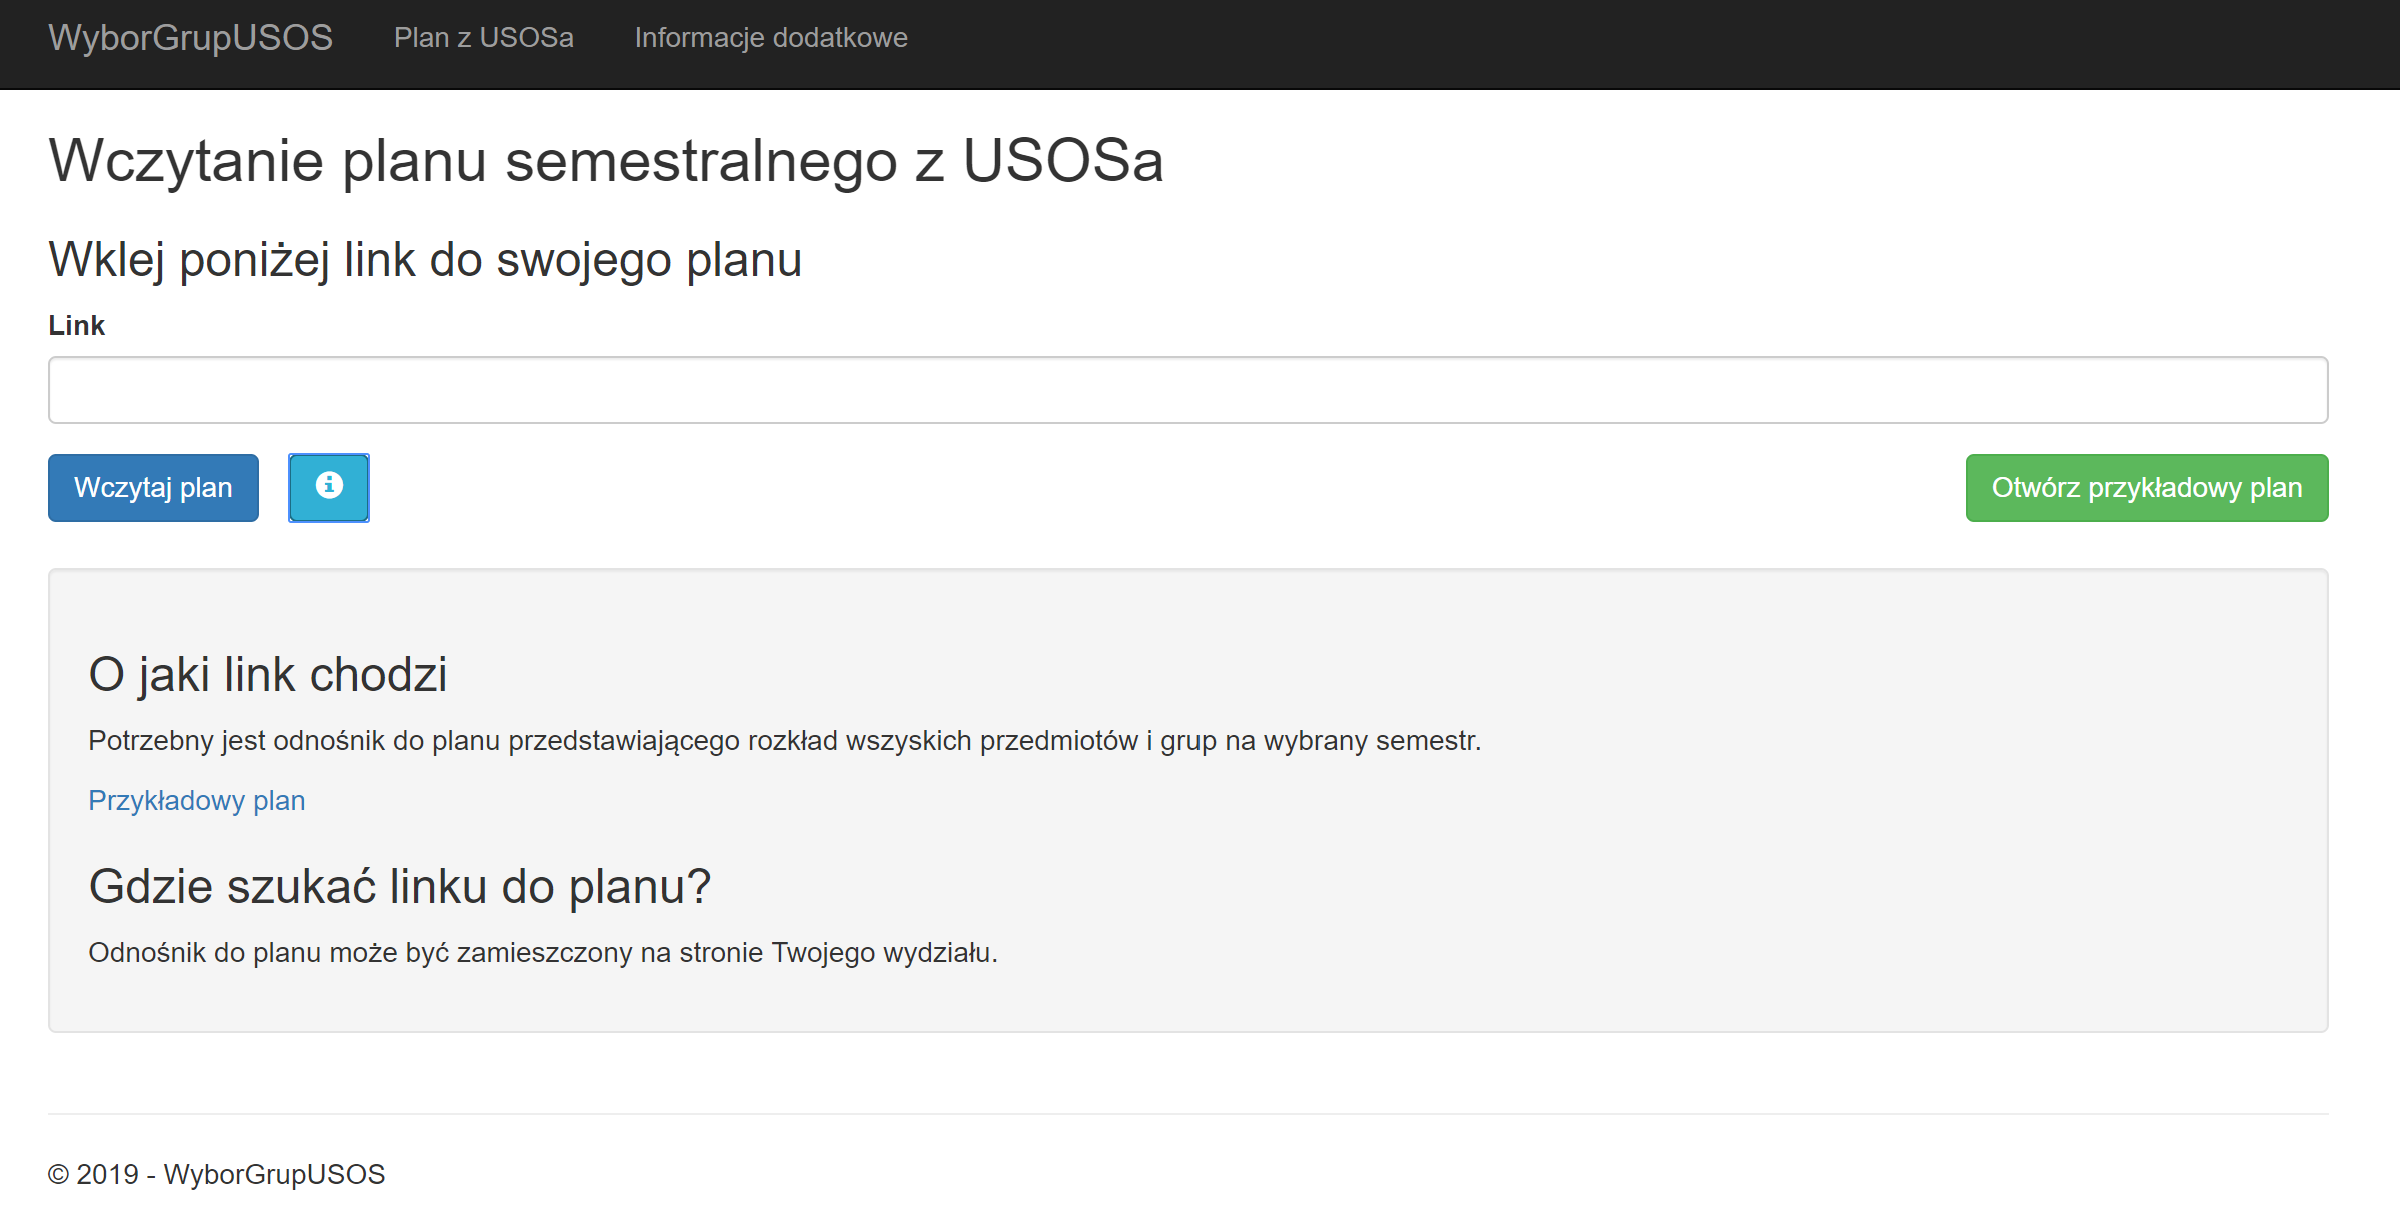
\includegraphics[width=13cm]{Ekran_wczytania_rozwiniety.png}
    \caption{Ekran wczytania z dodatkowymi informacjami}
    \label{fig:ekranWczytaniaRozwiniety}
\end{figure}

Po wczytaniu planu użytkownik zostanie przekierowany na ekran widoku planu. W górnej jego części znajduje się podgląd aktualnej konfiguracji plan. Na dole wyświetlane są kontrolki pozwalające na zmianę grupy. Przedmioty wyświetlane na planie są pokolorowane zgodnie z ich kategorią.

\begin{itemize}
    \item żółty -- ćwiczenia,
    \item niebieski -- wykład,
    \item różowy -- konwersatorium,
    \item czerwony -- \textbf{konflikt}.
\end{itemize}

Listy wyboru grup zawierają wartości wczytanie z planu. W sytuacji gdy więcej niż jedno zajęcie jest ustawione na wybraną godzinę pole zmieni dynamicznie kolor na czerwony.

Ekran ten przedstawia figura numer \ref{fig:ekranPlanu1}.

\begin{figure}[h]
    \centering
    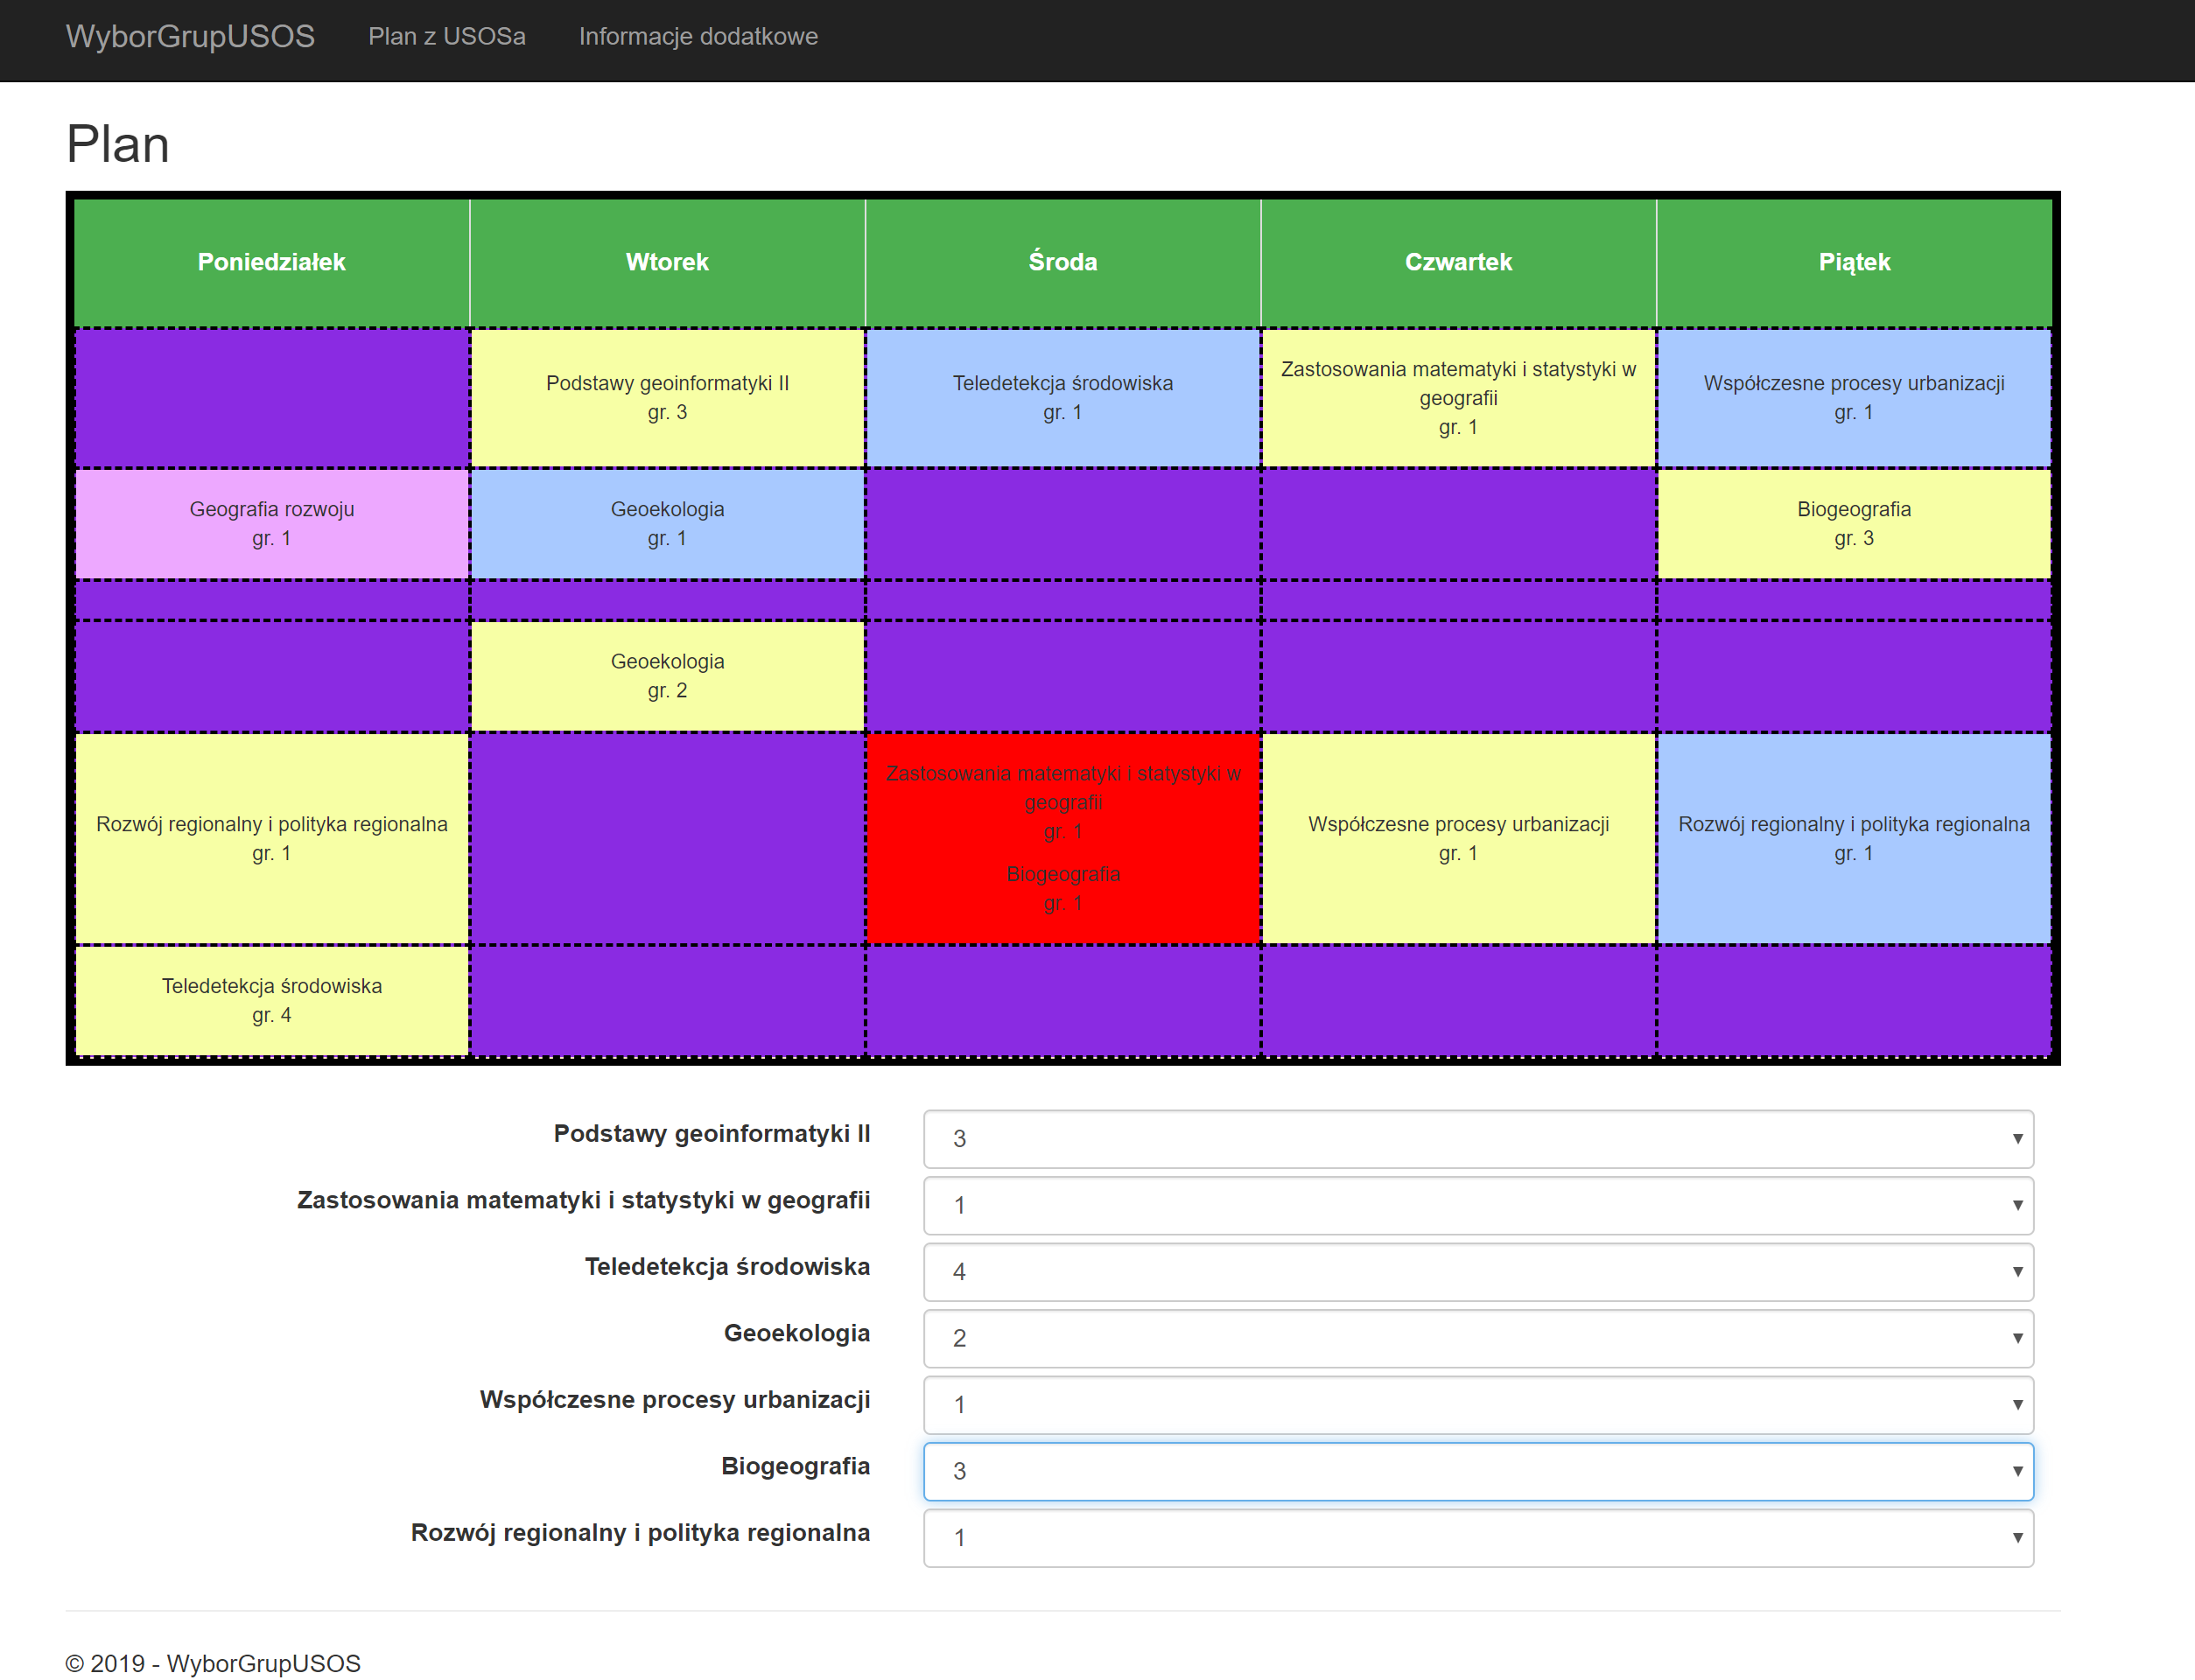
\includegraphics[width=13cm]{Wczytany_plan1.png}
    \caption{Ekran wczytania z dodatkowymi informacjami}
    \label{fig:ekranPlanu1}
\end{figure}


\section{Publikacja w chmurze} \label{sec:chmura}
W celu udostępnienie aplikacji w Internecie skonfigurowałem infrastrukturę w chmurze \textit{Microsoft Azure}. Dzięki temu aplikacja jest dostępna pod adresem \hyperlink{http://usos-plan.azurewebsites.net}{usos-plan.azurewebsites.net}.

\subsection{Podjęte kroki}
\begin{enumerate}
\item Założyłem subskrypcję studencką przy pomocy konta uczelnianego.
\item Utworzyłem grupę zasobów, powiązaną z subskrypcją, pozwalającą na łączne zarządzanie serwisami.
\item Skonfigurowałem \textit{App Service plan} tak by aplikacja była dostępna 24 godziny na dobę.
\item Utworzyłem \textit{App Service} pozwalający na przekazanie aplikacji webowej do chmury.
\item Wgrałem kod aplikacji do chmury przy pomocy środowiska \textit{Visual Studio}.
\end{enumerate}

Utworzona grupa zasobów jest pokazana na figurze \ref{fig:resourceGroup}

\begin{figure}[h]
    \centering
    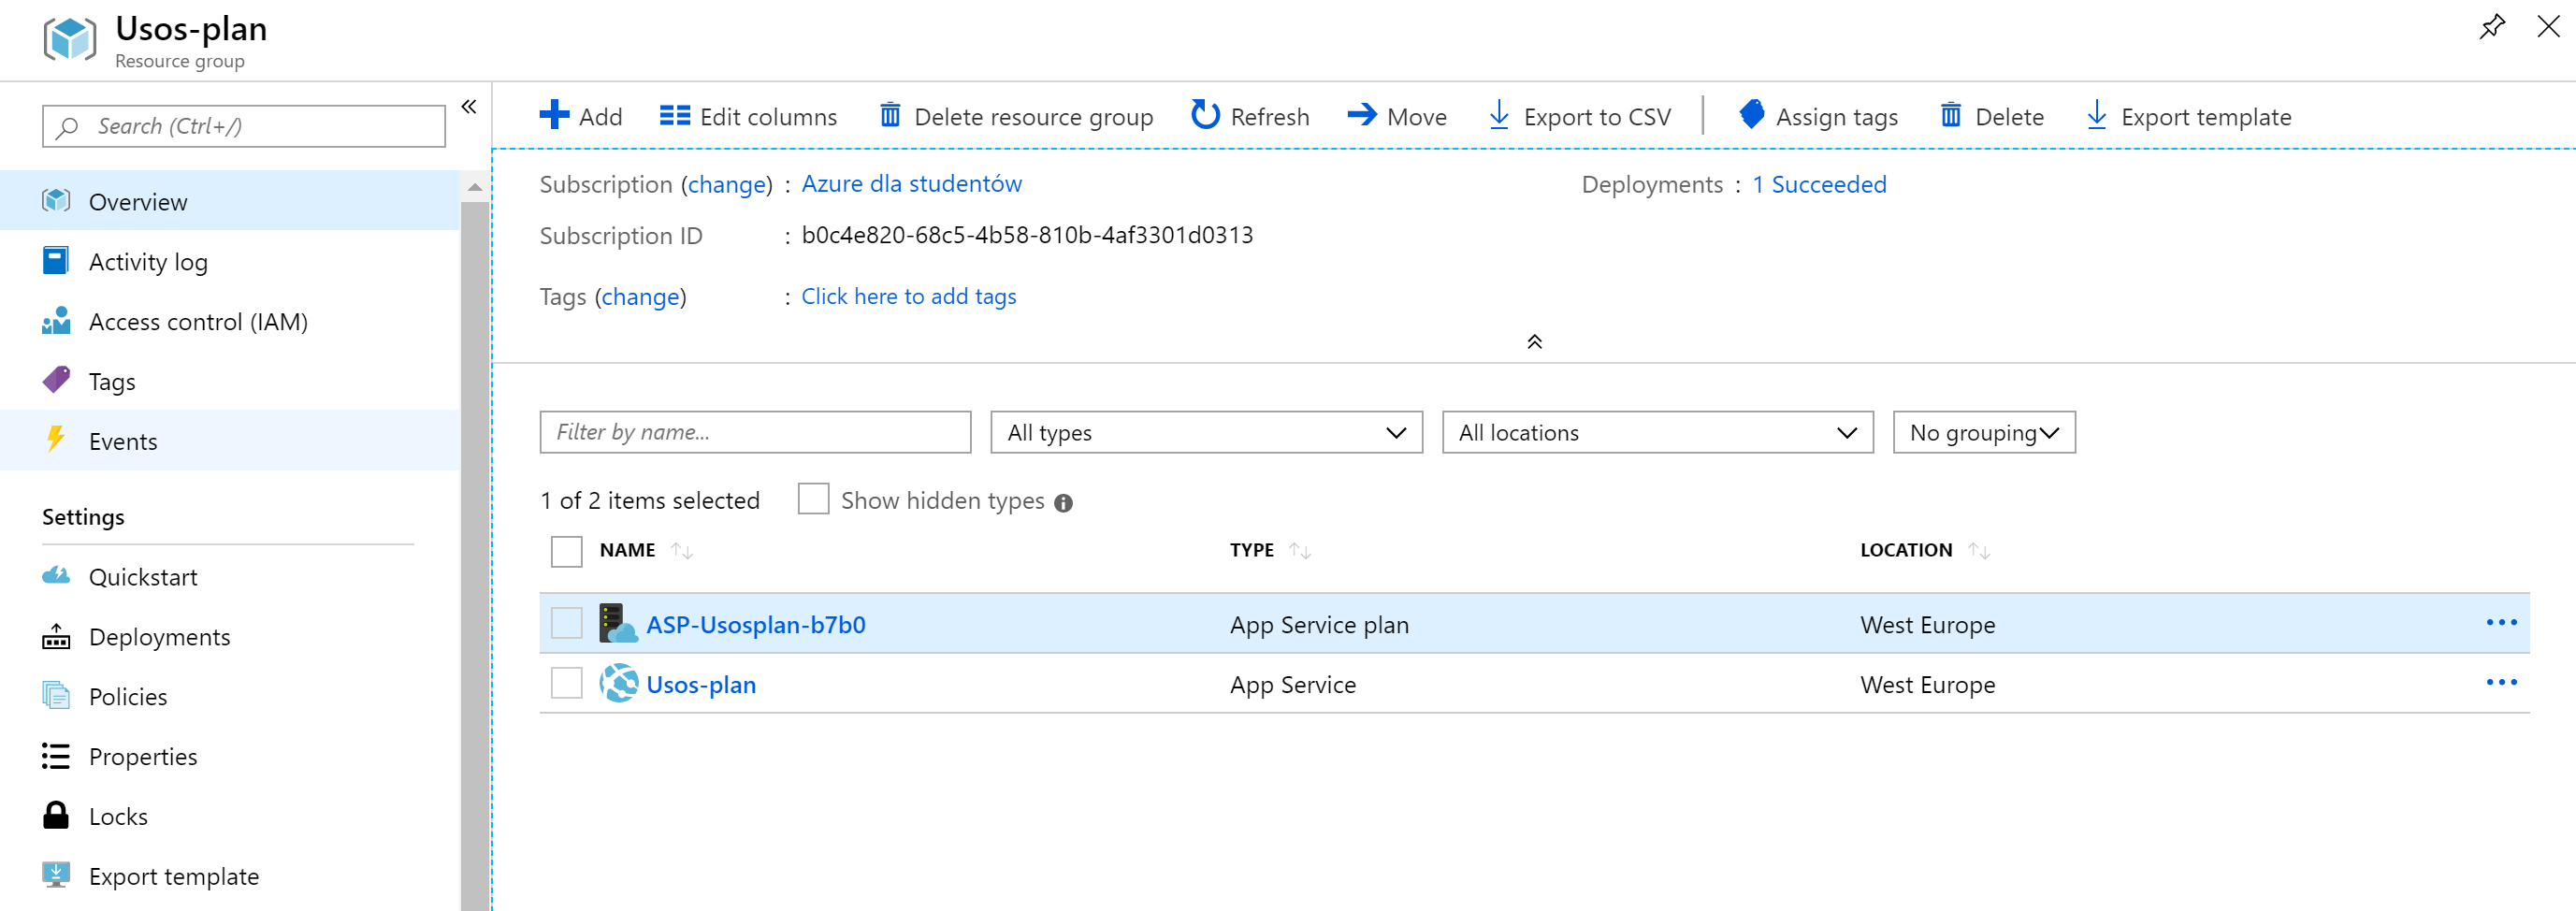
\includegraphics[width=13cm]{resource_group.png}
    \caption{Grupa zasobów na Azure}
    \label{fig:resourceGroup}
\end{figure}

\section{Szczegóły techniczne}

\subsection{Schemat działania}
Po wczytaniu linka wprowadzonego przez użytkownika modyfikowana jest część query string tak by otrzymać od serwisu \textit{USOS} cały plan w jednym pliku. Dzięki temu nie trzeba pobierać wielu stron opisjących szczegóły każdego z przedmiotów.

Następnie z odpowiedzi od serwera wyodrębniana jest tabela zawierająca plan. Jest ona parsowana wiersz po wierszu by określić informacje takie jak dzień, w którym organizowane są określone zajęcia. 

Po zakończeniu prasowania odpowiedzi serwera tworzony jest model planu zajęć. Na tym etapie wydzielane są grupy zajęć stanowiących wybór oraz zajęcia, na które student musi chodzić i nie ma żadnego wyboru.

Po utworzeniu modelu przekazywany jest on do widoku gdzie zgodnie ze wzorcem MVVM tworzony jest model widoku uwzględniający elementy takie jak aktualnie wygrane zajęcia dla każdej grupy.

Następnie model jest rysowany w postaci tabeli. W reakcji na zmianę grupy przez użytkownika model i wyświetlany widok są aktualizowane.

\subsection{Walidacja danych}
Lik wprowadzany przez użytkownika jest walidowany po stronie serwera. W tym celu zostały zastosowane adnotacje z przestrzeni nazw \texttt{System.ComponentModel.DataAnnotations}.

Sprawdzane jest czy wartość została wprowadzona adnotacją \texttt{Required} oraz poprawność linku adnotacją \texttt{RegularExpression}. Dzięki zastosowaniu tego rozwiązania mogą być automatycznie generowane odpowiednie komunikaty o błędach.

\subsection{Zastosowane mechanizmy}
Podczas pisania projektu poznałem wiele mechanizmów, które starałem się zastosować w projekcie.

\paragraphnl{linq}
Zastosowałem bibliotekę \texttt{linq} rozszerzającą metody kolekcji w celu filtrowania danych, mapowania oraz wybierania odpowiednich elementów ze zbirów.
Stosowałem za równo składnię \textbf{metod} jak i \textbf{zapytań}.

\paragraphnl{async}
Dzięki zastosowaniu programowania współbieżnego mogłem zwolnić aktualnie czekający wątek maszyny podczas wczytywania danych z zewnętrznych źródeł oraz zrównoleglić wykonywanie pracy.

\paragraphnl{Json.NET}
Przy pomocy tej biblioteki firmy \textit{Newtonsoft} mogłem z łatwością prasować i serializować obiekty do formatu JSON. Było to szczególnie przydatne przy konwersji modelu C\# na modle w języku JavaScript.

\paragraphnl{XPath}
Ponieważ dokument html jest poniekąd dokumentem xml to mogłem zastosować składnię XPath do wybierania odpowiednich elementów podczas przetwarzania odpowiedzi od serwisu \textit{USOS}.

\paragraphnl{Animacje CSS}
By nadać płynność elementowi ładowania pojawiającemu się podczas ładowania strony zastosowałem animacje opisywanie przez język CSS.
Opisują one w wektorowy sposób jakie transformacje mają zostać wykonane na obiekcie.

\paragraphnl{Wiązania danych}
Dzięki wiązaniom danych z biblioteki \textit{Knockout.js} można powiązać widok z modelem widoku realizując wzorzec MVVM. Pozwala to na dynamiczną aktualizację powiązanych wartości oraz na łatwe stosowanie wzorca Obserwator.

\section{Możliwości rozwoju}
W przyszłości do programu możnaby oddać następujące funkcjonalności.

\paragraphnl{Zapis stanu}
Do widoku planu można dodać przycisk pozwalający na zachowanie aktualnego ustawienia planu zajęć. W tym celu należałoby zapisać model widoku w bazie na serwerze. Aby to osiągnąć można zastosować blob storage z platformy \textit{Azure}.

\paragraphnl{Autmatyczne dopasowawnie konfiguracji planu}
Przydatny dla użytkownika mógłby okazać się algorytm, który automatycznie wybierałby grupy zajęć tak by osiągnąć wskazany przez użytkownika cel. Na przykład minimalizację okienek czy dopasowanie planu do grafiku pracy.

\paragraphnl{Wstawianie własnych zajęć}
Możliwość by użytkownik mógł dodawać własne dodatkowe zajęcia do wczytanego planu.

\paragraphnl{Usuwanie przedmiotów}
Możliwość by użytkownik mógł zrezygnować z wyświetlania zajęć z wybranego przedmiotu.

\paragraph{Konta użytkowników}
Dzięki systemowi logowań możaby powiązać dane takiej jak plany z poprzednich semestrów użytkownika czy zapisane konfiguracje z kontem danej osoby.

\end{document}

